% The vector overview spans both columns and is placed at the page top.
\begin{figure*}[t]
\centering
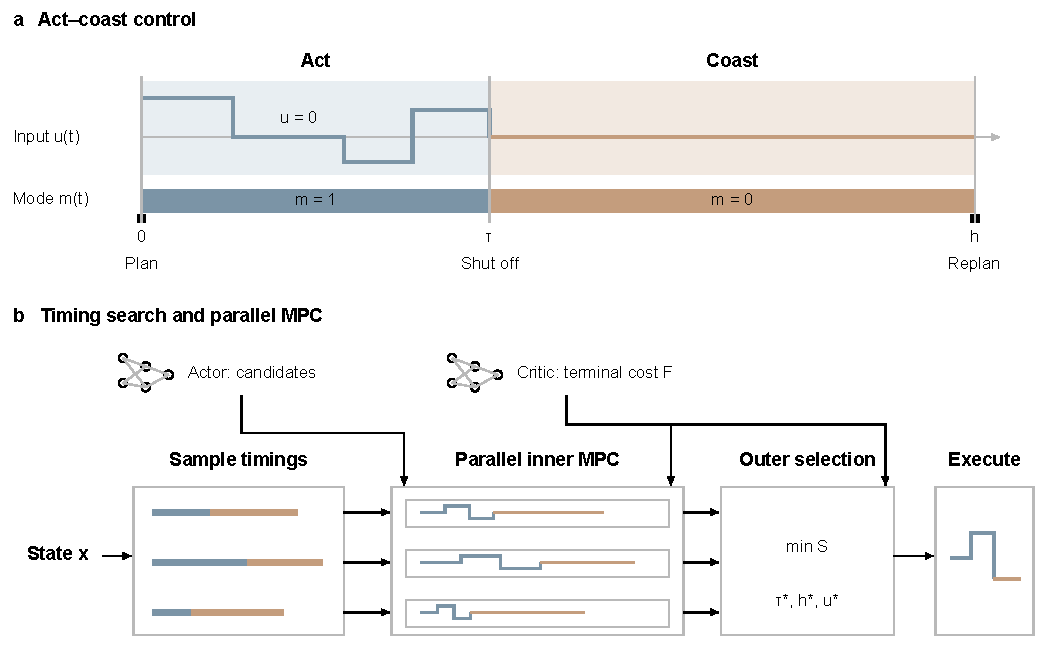
\includegraphics[width=\textwidth]{figures/act-coast-overview/figure-1-act-coast.pdf}
\caption{Act--coast concept and proposed controller construction.
(a) Time starts at the current decision. Input $u(t)$ executes planned commands until shut-off at $\tau$, then remains zero until replanning at $h$. Mode $m(t)$ is one during enabled operation and zero during coast, so an enabled zero command remains distinct from coast. Squares mark feedback decisions.
(b) At observed state $x$, outer MPC samples timing pairs $(\tau,h)$. One conditional inner MPC problem per pair optimizes the bounded input sequence; these problems are solved in parallel. The actor supplies candidates, and the critic-based terminal cost $F$ estimates actor continuation at each predicted replanning state. Thus $F$ influences both input optimization and the minimized event scores $S$ used for outer timing selection. The two critic arrows show this shared dependence; each event score includes its terminal cost once. Stars identify the selected times and input sequence $u^\star$. Miniature timing bars and input traces are schematic. The complete timing-conditioned construction remains to be evaluated.}
\label{fig:act-coast-overview}
\end{figure*}
